\documentclass[14px]{article}
\usepackage{xeCJK}
\usepackage[frenchb]{babel}
\usepackage[T1]{fontenc}
\usepackage[utf8]{inputenc}
\usepackage{textcomp}
\usepackage{amssymb}
\usepackage[ruled,longend]{algorithm2e}
\usepackage{amsmath}
\usepackage{latexsym}
\usepackage{fancyhdr}
\usepackage{geometry}
\usepackage{setspace}

% Image
\usepackage{graphicx}
\usepackage{subfigure}
\usepackage{caption}
\usepackage{float}
% wrap
\usepackage{wrapfig}
\usepackage[colorlinks,linkcolor=blue]{hyperref}

\renewcommand{\baselinestretch}{1.2}

\begin{document}
\setlength{\parindent}{0pt}
\begin{titlepage}

	\begin{center}
		% Upper part of the page
		
\includegraphics[width=0.35\textwidth]{logo.png}\\[1cm]

		\textsc{\Large Rapport du projet 1 de DAAR}\\[0.5cm]

		% Title

		{ \huge \bfseries Clone of the egrepDFA UNIX command}\\[0.4cm]

		% Author and supervisor
		\begin{minipage}{0.4\textwidth}
			\begin{flushleft} \large
				\emph{Rédacteurs:}\\
				Qiwei \textsc{XIAN}\\
				Mehdi-Nassim \textsc{KHODJA}
			\end{flushleft}
		\end{minipage}
		\begin{minipage}{0.4\textwidth}
			\begin{flushright} \large
				\emph{Professeur:} \\
				Prof.\textsc{Bui-Xuan}
			\end{flushright}
		\end{minipage}

		\vfill
		% Bottom of the page
		{\large \today}
	\end{center}

\end{titlepage}
\clearpage

\tableofcontents
\thispagestyle{empty}
\clearpage

\pagestyle{fancy}
\lhead{Objectif}

\rhead{\thepage}
\fancyfoot{}

\section{Préface}
\subsection{Objectif}
L'objectif du projet est de chercher tous les lignes qui contiennent les mots correspondant à l'expression régulière saisie. Nous devons comprendre comment transformer l'expression régulière à l'automate fini déterministe minimale correspondante.

\subsection{Définition}
\subsubsection{Définition des termes utilisés}
\begin{enumerate}
	\item RET (Regular Expression Tree) : l'arbre de l'expression régulière.
	\item DFA (Deterministic finite automaton) : l'automate fini déterministe
	\item NFA (Nondeterministic finite automaton) : l'automate fini non déterministic
\end{enumerate}

\subsubsection{Définition des structure de données}
\begin{enumerate}
	\item RegExTree : Il représent chaque noeud de l'arbre de l'expression régulière, l'attribut root est l'opérator ou une lettre, subTrees est une liste des noeuds fils. 
	\item Node : Cette structure de données représente chaque noeud de l'automate, il contient un hashmap qui permet de stocker les étiquettes des lien ainsi que les voisins.
	\item Automaton : Cette structure possède le noeud initial et une liste des noeuds.     
\end{enumerate}

\section{Algorithme}
Pour construire un DFA minimale par RET, il y a 3 étapes: La transformation de RET à NFA, celle de NFA à DFA, la minimization de DFA. 

\subsection{Transformation de RET à NFA}
On d'abord observe la strucutre de RET, on peut savoir que le noeud représente l'opérator si et seulement si c'est un noeud interne, sinon il représente une lettre.

Donc on parcourt RET en suffix, on arrive d'abord les noeuds feuilles et construit l'automate de base, comme l'image\ref{img1}. Ensuite on arrive les noeuds internes et on connecte l'automate de fils gauche et de fils droite par le lien epsilon en fonction de l'opérator actuel. Il y a 2 formes différente de connection, la concaténation et l'alternance, l'image\ref{img2}. En plus une connection spéciale pour l'opérateur étoile. Le noeud interne dont root est l'étoile ne possède qu'un noeud fils dans ce cas, comme l'image\ref{img4}.

Une fois qu'on fait cette étape, on peut obtenir un NFA avec des lien epsilon. Pour les codes de source, la réalisation de cette étape est la fonction $parse(RegExTree regTree)$.

\subsection{Transformation de NFA à DFA}
Dans cette étape, on élimine les liens epsilon et mélanger les noeuds qui sont dans le même groupe. On note que l'ensemble de noeuds $\mathcal{P}$.
\subsubsection{Création des noeuds nouvelle pour DFA}
L'idée est simple, on cherche d'abord les noeuds qui ne reçoivent pas le lien d'epsilon dans $\mathcal{P}$ et on note ces noeuds $S$. Par exemple, pour NFA\ref{img5}, les noeuds 0,2,5 et 8 qui ne reçoivent pas de lien epsilon.

Pour chaque noeud de $S$, on crée un nouveau noeud. On va obtenir une nouvelle ensemble $S^{\prime}$, on construit un hashmap qui permet de trouver noeud de $S^{\prime}$ par celui de $S$ à la fois, on note $hashmap[s] = s^{\prime}, s \in S, s^{\prime} \in S^{\prime}$. DFA sera composé par les noeuds de $S^{\prime}$.

\subsubsection{Addition des liens dans DFA}
Ensuite, pour chaque noeud $s, s \in S$, on fait un DFS, lors qu'on arrive un autre noeud $s^{\prime}, s^{\prime} \in S$ via le lien $l$, on ajoute le lien $l$ entre le noeud $hashmap[s]$ et $hashmap[s^{\prime}]$. Si on arrive une noeud final par un lien epsilon, on marque que $hashmap[s]$ est aussi final.\\

Après cette étape, tous les liens non epsilon sont ajoutés dans DFA. Pour nos codes de source, la réalisation de cet algorithme est la fonction $transformNFAToDFA(Automaton NFA)$.

\subsection{Minimization de DFA : Hopcroft}
On a utilisé l'algorithme de Hopcroft pour minimiser DFA actuel. L'idée de minimization est classifier les noeuds en m groupes $(m < n, n == |\mathcal{S}|)$, jusqu'à on ne peut plus continuer de séparer. Ensuite on connecte ces m groupes, alors DFA est minimizé.

\subsubsection{Classification des noeuds}
La principe de classification est mettre les noeuds équivalents dans le même groupe. Si les successeurs de deux noeuds sont dans le même groupe, alors on dit que ces deux noeuds sont équivalent.

On sépare initialement $\mathcal{S}$ en deux groupes, $A$ pour les noeuds acceptables, $B$ pour ceux non acceptables. Pour chaque noeud de groupe, on vérifie si ses successeurs sont dans le groupe où il se trouve, sinon on met ce noeud dans un nouveau groupe. Après plusieur tours de séparation, on ne peut plus continuer à séparer, la classification est terminée.

La réalisation de cette étape est la fonction $classifyNode$.

\subsubsection{Construction DFA minimal}
Une fois qu'on fait la classification, il y a $m$ groupes. On crée un nouveau noeud pour chaque groupe, et note eux $M$. DFA minimal se compose des noeuds de $M$. Le hashmap $h$ est aussi construit, on déclare $h[s] = m, m \in M, s \in S$.

On parcourt DFA précédent par BFS, pour le noeud actuel $cur$, si le successeur de $cur$ (on note $suc$) appartient à un autre groupe, alors on connecte $h[cur], h[suc]$ par le lien entre $cur$ et $suc$. Sinon on continue le processus de BFS. Après BFS, DFA minimal est bien complété. 

La réalisation de cette étape est la fonction $minimize(Automaton DFA)$.

\subsection{Réalisation de commande egrepDFA}
Pour cette étape, on applique simplement le générateur de DFA minimal dans la copie de egrepDFA. Pour chaque ligne de l'article. On appelle une fois $DFA.search(ligne)$. Si il peut arriver le noeud acceptable de DFA, alors on rend cette ligne.

\subsection{Figures}
\begin{figure}[H]
	\begin{minipage}[H]{0.3\linewidth}
		\centering
		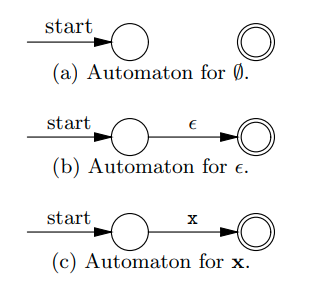
\includegraphics[width=\textwidth]{AutomateBase.png}\\
		\caption{Automate de base}
		\label{img1}
	\end{minipage}
	\begin{minipage}[H]{0.4\linewidth}
		\centering
		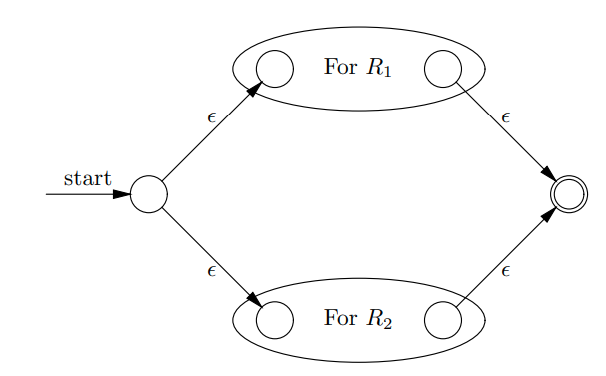
\includegraphics[width=\textwidth]{Connection1.png}
		\caption{Connection d'alternance}
		\label{img2}
	\end{minipage}
\end{figure}
\begin{figure}[H]
	\begin{minipage}[H]{0.4\linewidth}
		\centering
		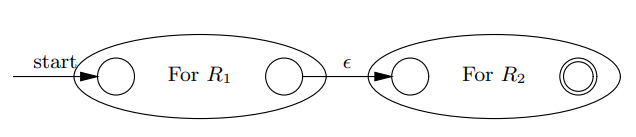
\includegraphics[width=\textwidth]{Connection2.png}
		\caption{Connection de concatenation}
		\label{img3}
	\end{minipage}
	\begin{minipage}[H]{0.4\linewidth}
		\centering
		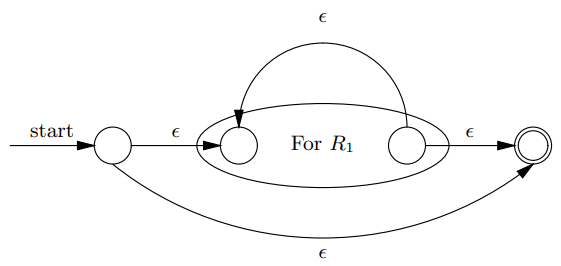
\includegraphics[width=\textwidth]{Connection3.png}\\
		\caption{Connection de closure}
		\label{img4}
	\end{minipage}
\end{figure}

\begin{figure}[H]
	\begin{minipage}[H]{0.8\linewidth}
		\centering
		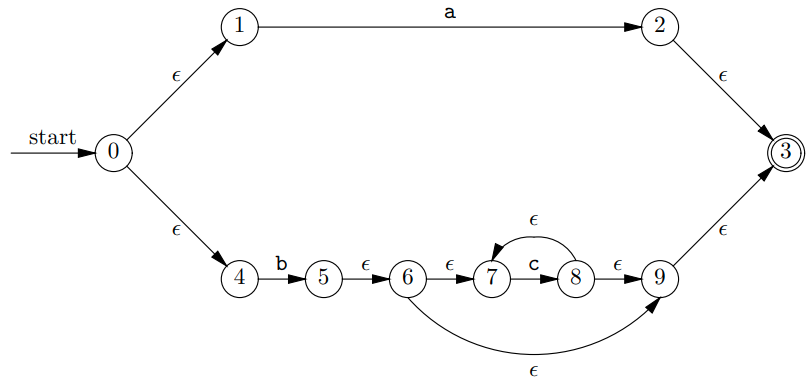
\includegraphics[width=\textwidth]{exempleAutomate.png}\\
		\caption{Une exemple de NFA}
		\label{img5}
	\end{minipage}
\end{figure}




\section{Analyse de complexité}
\subsection{Cas général}
Dans le cas général, DFA permet de trouver tous les lignes qui contient le mot satisfaisant à l'expression régulière saisie. Supposons que la longueur de chaine de caractères est $n$, pour vérifier si elle contient le mot suffisant, on a besoin d'appeler n fois $DFA.search(str.substr(i, n))$, i est l'indice du commencement, $i \in [0, n]$, dans le pire cas. Donc la complexité est $\frac{(1 + n) * n}{2} = \mathcal{O}(n^{2})$.

\subsection{Cas particulière}
Le cas particulier est qui l'expression régulière saisie est seulement une chaine de caractère. Dans ce cas-là, on n'a plus besoin de construire DFA, la solution optimale est l'algorithme KMP. Cela permet de résoudre le problème en $\mathcal{O}(n)$.


\section{Partie de test}
Rédacteur : mehdi. l'explication de résultat de l'exécution, tu peux mettre une capture d'écran dans la section Annexe, et utiliser ref pour redirect à la position des images, comme ce que j'ai fait au dessus.

\section{Test de performance}
Rédacteur : mehdi. tu compares le temps d'exécution des cas différents.

\section{conclusion}
L'utilisation de DFA peut garantir une complexité de base $O(n^{2})$ pour vérifier si une chaine de caractère qui contient le mot satisfaisant à l'expression régulière saisie. L'algorithme KMP peut optimiser certain cas particulier.


\end{document}
